\chapter{\mysketch}
\label{chap:quancurrent}

We present \mysketch, an $r$-relaxed concurrent Quantiles sketch where $r$ depends on system parameters as discussed below. The algorithm uses $N$ update threads to ingest stream elements and allows an unbounded number of query threads. Queries are processed at any time during the sketch's construction. 
We consider a shared memory model that provides synchronization variables (atomics) and atomic operations to guarantee sequential consistency as in C++~\cite{Boehm_2008_cpp}. Everything that happened-before a write in one thread becomes visible to a thread that reads the written value. Also, there is a single total order in which all threads observe all modification in the same order. 
We use the following sequentially consistent atomic operations (which force a full fence): \emph{fetch-and-add (F\&A)}~\cite{x86-faa} and \emph{compare-and-swap (CAS)}~\cite{x86-cas}. 

In addition, we use a software-implemented higher-level primitive, \emph{double-compare-double-swap (DCAS)} which atomically updates two memory addresses as follows: DCAS($addr_1$: $old_1 \to new_1$, $addr_2$: $old_2 \to new_2$)
is given two memory addresses $addr_1$, $addr_2$, two corresponding expected values $old_1$, $old_2$, and two new values $new_1$, $new_2$ as arguments. It atomically sets $addr_1$ to $new_1$ and $addr_2$ to $new_2$ only if both addresses match their expected values, i.e., the value at $addr_1$ equals $old_1$ and the value at $addr_2$ equals $old_2$. DCAS also provides wait-free DCAS\_READ primitive, which can read fields that are concurrently modified by a DCAS. DCAS can be efficiently implemented using single-word CAS~\cite{Harris2002practical,guerraoui2020efficient}. 


In Section~\ref{sec:data_org}, we present the data structures used by Quancurrent. Section~\ref{sec:update_alg} presents the update operation, and \todo[color=red]{fix} Section~\ref{sec:query_alg} presents the query. The formal correctness proof is deferred to the supplementary material. 


\section{Data Structures} \label{sec:data_org}

\mysketch's data structures are described in Algorithm~\ref{alg:data_organization} and depicted in Figure~\ref{fig: data_structures}.
Similarly to the sequential Quantiles sketch, \mysketch is organized as a hierarchy of arrays called \emph{levels}. Each level can be \emph{empty}, \emph{full}, or in \emph{propagation}. The variable \emph{tritmap} maintains the states of all levels. Tritmap is an unsigned integer, interpreted as an array of trits (trinary digits). The trit $tritmap[i]$ describes level $i$'s state: if $tritmap[i]$ is $0$, level $i$ contains $0$ or $2k$ ignored elements and is considered to be empty. If $tritmap[i]$ is $1$, level $i$ contains $k$ elements and is deemed full, and if it is $2$, level $i$ contains $2k$ elements and is associated with the propagation state. Each thread has a local buffer of size $b$, $\mathit{localBuf[b]}$. Before ingested into the sketch's levels, stream elements are buffered in threads local buffers and then moved to a processing unit called $\mathit{Gather\&Sort}$. The $\mathit{Gather\&Sort}$ object has two $2k$-sized shared buffers, $\mathit{G\&SBuffer}[2]$, each with its own $\mathit{index}$ specifying the current location, as depicted in Figure~\ref{fig: gather_and_sort}. 

The query mechanism of \mysketch includes taking an atomic snapshot of the levels. Query threads cache the snapshot and the tritmap that represents it in local variables, 
$\mathit{snapshot}$ and $\mathit{myTrit}$, respectively. As the snapshot reflects only the sketch's levels and not G\&SBuffers or the thread's local buffers, Quancurrent is ($4kS+(N-S)b$)-relaxed Quantiles sketch where $S$ is the number of NUMA nodes. 


\begin{algorithm}[h]
\caption{\mysketch data structures} \label{alg:data_organization}
    \begin{algorithmic}[1] 
    \setcounter{ALG@line}{\value{mycounter}}
    \State \textbf{Parameters and constants:}
        \State \hspace{\algorithmicindent} \myvar{MAX\_LEVEL} 
        \State \hspace{\algorithmicindent} \myvar{k} \Comment{sketch level size}
        \State \hspace{\algorithmicindent} \myvar{b} \Comment{local buffer size}
        \State \hspace{\algorithmicindent} \myvar{S} \Comment{\#NUMA nodes}
    \State
    \State \textbf{Shared objects:} \;
        \State \hspace{\algorithmicindent} \myvar{tritmap} $\gets 0$ 
        \State \hspace{\algorithmicindent} \myvar{levels}[\myvar{MAX\_LEVEL}]
    \State
    \State \textbf{NUMA-local objects:} \Comment{shared among threads on the same node}
        \State \hspace{\algorithmicindent} \myvar{G\&SBuffer}[2][2\myvar{k}]
        \State \hspace{\algorithmicindent} \myvar{index}[2] $\gets \{0,0\}$
    \State
    \State \textbf{Thread local objects:}
        \State \hspace{\algorithmicindent} \myvar{localBuf}[\myvar{b}]
        \State \hspace{\algorithmicindent} \myvar{myTrit} \Comment{used by query}
        \State \hspace{\algorithmicindent} \myvar{snapshot} \Comment{used by query}
        \setcounter{mycounter}{\value{ALG@line}}
    \end{algorithmic}
\end{algorithm}

%============================================================
\section{Update} \label{sec:update_alg} %Blocking, Holes, Double Base Buffer, Sorted Local Buffers Update, Merge using k-Way Merge Sort
%============================================================
The ingestion of stream elements occurs in three stages: 
(1) \emph{gather and sort}, 
(2) \emph{batch update}, and 
(3) \emph{propagate level}. 
In stage (1), stream elements are buffered and sorted into batches of $2k$ through a $\mathit{Gather\&Sort}$ object. Each NUMA node has its designated $\mathit{Gather\&Sort}$ object, which is accessed by NUMA-local threads. 
Stage (2) executes a batch update of $2k$ elements from the $\mathit{Gather\&Sort}$ object to $levels[0]$. 
Finally, in stage (3), $levels[0]$ is propagated up the levels of the hierarchy.

%============================================================
% \subsubsection{Stage 1: Gather and Sort} \label{Section: part1_update} 
%============================================================
In the first stage, threads first process stream elements into a thread-local buffer of size $b$. Once the buffer is full, it is sorted and the thread reserves $b$ slots on a shared buffer in its node's Gather\&Sort unit. It then begins to move the local buffer's content to the shared buffer. The shared Gather\&Sort buffer contains $2k$ elements, and its propagation (during Stage 2) is not synchronized with the insertion of elements. Thus, some reserved slots might still contain old values, (which have already been propagated), instead of new ones. As the batch is a sample of the original stream, we can accept the possible loss of information in order to improve performances. Below, we show that the sampling bias this introduces is negligible.

The pseudo-code for the first stage is presented in Algorithm~\ref{alg:gather}. To insert its elements to the shared buffer, a thread tries to reserve $b$ places in one of the shared buffers using F\&A (Line~\ref{Line: fetch_idx}). If the index does not overflow, the thread copies its local buffer to the reserved slots (Line~\ref{Line: copy_local_buffer}). We refer to the thread that fills the last $b$ locations in a G\&SBuffer as the \emph{owner} of the current batch. The batch owner creates a local sorted copy of the shared buffer and begins its propagation (Lines~\ref{Line:create_copy}-\ref{Line:call_batchUpdate}).

Note that the local buffer is not atomically moved into the shared buffer (Line \ref{Line: copy_local_buffer} is a loop). Thus, the owner might begin a propagation before another thread has finished moving its elements to the shared buffer. In this case, the old elements already contained within the G\&SBuffer are taken instead. Furthermore, upon moving its elements later, the writer thread might overwrite more recent elements. In other words, during this stage, stream elements may be duplicated and new elements may be dropped. We call both of these occurrences \emph{holes}, and analyze their implications in Section~\ref{ssec:holes-analysis} \todo[color=red]{fix}.


\begin{algorithm}[h]
\caption{Stage 1: gather and sort} \label{alg:gather}
% \alglanguage{algpseudocode}
\begin{algorithmic}[1]
\setcounter{ALG@line}{\value{mycounter}}
\Procedure{update}{$x$}
    \State add $\mathit{x}$ to \myvar{localBuf} \Comment{thread-local} \label{Line: update_linearization}
    \If{$\neg \mathit{localBuf}$.full()}
        \State \Return
    \EndIf
    \State sort \myvar{localBuf}
    \State \myvar{i} $\gets 0$
    \While{\textbf{true}} \Comment{insert to Gather\&Sort unit}
        \State \myvar{idx} $\gets$ \myvar{index}[\myvar{i}].F\&A(\myvar{b}) \label{Line: fetch_idx}
        \If{$\mathit{idx}< 2k$}
            \State move \myvar{localBuf} to \myvar{G\&SBuffer}[\myvar{i}][$\mathit{idx}, \dots, \mathit{idx}+b$] \label{Line: copy_local_buffer}
            \If{$\var{idx}+b=2k$} \Comment{owner, filled buffer}
                \State $\mathit{myCopy} \gets \text{sorted copy of } \mathit{G\&SBuffer}[\mathit{i}]$ \label{Line:create_copy}
                \State batchUpdate(\myvar{i},\myvar{myCopy}) \label{Line:call_batchUpdate}
            \EndIf
            \State \Return
        \EndIf
        \State \myvar{i} $\gets$ $\neg$\myvar{i}
    \EndWhile
\EndProcedure
\setcounter{mycounter}{\value{ALG@line}}
\end{algorithmic}
\end{algorithm}



\begin{figure}[h]
    \begin{subfigure}[b]{\linewidth}
    \centering
    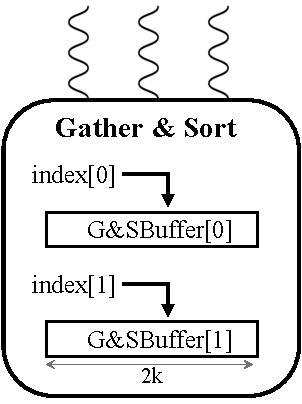
\includegraphics[width=0.3\linewidth]{graphics/algorithm/gather_and_sort.pdf}
    \caption{$\mathit{Gather\&Sort}$ object.}
    \label{fig: gather_and_sort}
    \end{subfigure}
    % \vfill
    \par\medskip
    \begin{subfigure}[b]{\linewidth}
    \centering
    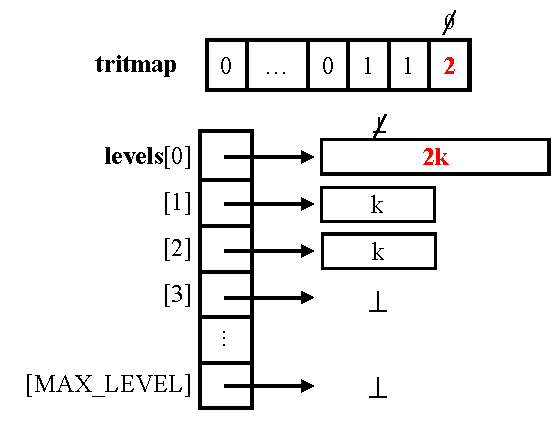
\includegraphics[width=0.5\linewidth]{graphics/algorithm/batch_update.pdf}
    \caption{Batch update into $\mathit{levels}[0]$.}
    \label{fig: batch_update}
    \end{subfigure}%
    
    \caption{Quancurrent's data structures.}
    \label{fig: data_structures}
\end{figure}




%============================================================
% \subsubsection{Stage 2: Batch Update} \label{Section: part2_batch_update}
%============================================================
In the second stage, the owner inserts its local sorted copy of the shared buffer into level $0$ using a DCAS. The batch of $2k$ elements is only inserted when level $0$ is empty, reflected by the first digit of the tritmap being $0$. We use DCAS to atomically update both \emph{levels}[0] to point to the new sorted batch and \emph{tritmap} to indicate an ongoing batch update (reflected by setting $\mathit{tritmap[0]}$ to 2). The DCAS might fail if other owner threads are trying to insert their batches or propagate them. The owner keeps trying to insert its batch into the sketch's first level until a DCAS succeeds, and then resets the index of the G\&SBuffer to allow other threads to ingest new stream elements. 
The pseudo-code for the second stage is presented in Algorithm~\ref{alg: batch_update}, and an example is depicted in Figure~\ref{fig: batch_update}.

\begin{algorithm}
\caption{Stage 2: batch update} \label{alg: batch_update}
\begin{algorithmic}[1]
\setcounter{ALG@line}{\value{mycounter}}
\Procedure{batchUpdate}{\myvar{i},\myvar{base\_copy}}
    \While{$\neg$DCAS(\myvar{levels}[0]: $\bot \to$ \myvar{base\_copy}, \myvar{tritmap}[0]: 0 $\to$ 2} \label{Line:insert_batch}
        \State \myvar{index}[\myvar{i}] $\gets 0$
        \State propagate(0)
    \EndWhile
\EndProcedure
\setcounter{mycounter}{\value{ALG@line}}
\end{algorithmic}
\end{algorithm}


%============================================================
% \subsubsection{Stage 3: Propagate Level} \label{Section: part3_propagate} 
%============================================================
In the beginning of the third stage, level 0 points to a new sorted copy of a \emph{G\&SBuffer} array and \emph{tritmap}[0]=2. During this stage, the owner thread propagates the newly inserted elements up the levels hierarchy iteratively, level by level from level 0 until an empty level is reached. The pseudo-code for the propagation stage is presented in Algorithm~\ref{alg: propagate}. On each call to \emph{propagate}, level $l$ is propagated to level $l+1$, assuming that level $l$ contains $2k$ sorted elements and $\mathit{tritmap}[l]=2$. If $\mathit{tritmap}[l+1]=2$, the owner thread is blocked by another propagation from $l+1$ to $l+2$ and it waits until $\mathit{tritmap}[l+1]$ is either a $0$ or $1$. The owner thread samples $k$ elements from level $l$ and retains the odd or even elements with equal probability (Line~\ref{Line: choose_rand}). 
If $\mathit{tritmap}[l+1]$ is $1$, then level $l+1$ contains $k$ elements. The sampled elements are merged with level $l$+1 elements into a new $2k$-sized sorted array (Line~\ref{Line: next_full}). We then (in Line~\ref{Line:next_full_DCAS}) continuously try, using DCAS, to update \emph{levels}[$l$+1] to point to the merged array and atomically update \emph{tritmap} such that \emph{tritmap}[$l$] $\gets 0$, reflecting level $l$ is available, and \emph{tritmap}[$l$+1] $\gets 2$, reflecting that level $l$+1 contains $2k$ elements. After a successful DCAS, we clear level $l$ (set it to $\bot$) and proceed to propagate the next level (Line~\ref{Line:propagate_next}). 
If $\mathit{tritmap}[l+1]$ is $0$, then level $l+1$ is empty. We use DCAS (Line~\ref{Line:next_empty_DCAS}) to update $\mathit{levels}[l+1]$ to point to the sampled elements and atomically update \emph{tritmap} so that \emph{tritmap}[$l$] becomes $0$, and \emph{tritmap}[$l$+1] becomes $1$ (containing $k$ elements). After a successful DCAS, we clear level $l$ (set it to $\bot$) and end the current propagation.

Propagations of different batches may occur concurrently, i.e., level propagation of levels $l$ and $l'$ can be performed in parallel. Figure~\ref{fig: propagate} depicts an example of concurrent propagation of two batches.


% \begin{algorithm}[h]
% \caption{Stage 3: Propagation of level $l$} \label{alg: propagate}
% \SetKwFunction{propagate}{propagate}
% \Procedure{\propagate{\myvar{l}}}{
%     %\Comment*[l]{\myvar{tritmap}[\myvar{l}] was set to 2 by this thread and wasn't changed}
%     \lIf(){\myvar{l} $\geq$ \myvar{MAX\_LEVEL}}{\KwRet{}}
%     \Comment*[l]{choose odd or even indexed elements randomly}
%     \myvar{newLevel} $\gets$ sampleOddOrEven(\myvar{levels}[\myvar{l}]) \; \label{Line: choose_rand}
%     \uIf(\Comment*[f]{next level is full}){\myvar{tritmap}[\myvar{l}$+1$] $ =1$}{
%          \myvar{newLevel} $\gets$ merge(\myvar{newLevel}, \myvar{levels}[\myvar{l}$+1$]) \label{Line: next_full}\;
%          \lWhile(\label{Line:next_full_DCAS}){$\neg$DCAS(\myvar{levels}[\myvar{l}$+1$]: \myvar{levels}[\myvar{l}$+1$] $\to$ \myvar{newLevel},  \myvar{tritmap}[\myvar{l}, \myvar{l}$+1$]: $ [2,1] \to [0,2]$)}{\{ \}} 
%         \myvar{levels}[\myvar{l}] $\gets \bot$ \Comment*[r]{clear level} 
%         \KwRet{propagate(\myvar{l}+1)} \label{Line:propagate_next}
%     }
%     \Comment*[l]{\myvar{tritmap}[\myvar{l}+1] is 0 or 2}
%     \lWhile(\label{Line:next_empty_DCAS}){$\neg$DCAS(\myvar{levels}[\myvar{l}$+1$]: $ \bot \to$ \myvar{newLevel}, \myvar{tritmap}[\myvar{l}, \myvar{l}$+1$]: $ [2,0] \to [0,1]$)}{\{ \}} 
%         \myvar{levels}[\myvar{l}] $\gets \bot$ \Comment*[r]{clear level} 
% }
% \end{algorithm}

\begin{figure*}[h]
\includegraphics[width=0.8\textwidth,trim={0 0cm 0 0},clip]{images/Quancurrent/propagate short.pdf}
\centering
\captionsetup{justification=centering}
\caption[\mysketch~\xspace propagation.]{\mysketch~\xspace propagation. \par \small \textbf{(a)} The owner of batch $i$, owner($i$), inserts batch $i$ to level $0$ and atomically updates $tritmap[0]$ to $2$. 
\textbf{(b)} owner($i$) merges level $0$ with level $1$ and changes $tritmap[1,0]$ from $[1,2]$ to $[2,0]$. 
\textbf{(c)} owner($i$) clears level $0$. 
\textbf{(d)} owner($i+1$) inserts its batch to level $0$ and atomically updates $tritmap[0]$ to $2$. 
\textbf{(e)} owner($i$) merges level $1$ with level $2$, and sets $tritmap[2,1]$ to $[2,0]$. Batch $i+1$ is still blocked because level $1$ has not been cleared yet. 
\textbf{(f)} owner($i$) clears level $1$. 
\textbf{(g)} Now owner($i+1$) successfully merges level $0$ with the empty level $1$, and sets $tritmap[1,0]$ to $[1,0]$. 
}
\label{fig: propagate}
\end{figure*}
